\documentclass{article}
\usepackage[pdfusetitle,pdflang=en-UK]{hyperref}
\usepackage{graphicx} % Required for inserting images
%\usepackage[sort&compress,numbers]{natbib}
%\usepackage{pdfcomment}
%\usepackage{amsmath}
\renewcommand{\familydefault}{\sfdefault}
\usepackage[a4paper, total={6in, 8in}]{geometry}
\usepackage[UKenglish]{datetime}
\usepackage[tagged, highstructure]{accessibility}


\title{Accelerating Molecular Dynamics with Machine Learning \\ Workshop 4, SFB 986 Spring School 2024}
\author{Alan M. Lewis}

\date{}

\begin{document}

\maketitle

\section{Getting Started}

%This workshop is designed to be completed in groups of 2-4. Try to ensure your group has a mix of people with and without experience in coding, so you can help each other. If someone in the group is unable to run one or both machine learning packages, they are responsible for plotting graphs of the data produced by the other team members. Each section has subsections which should be completed by everybody, and subsections which can be divided amongst the group. These should be clearly indicated.

To get started, if you are running Ubuntu, open a command line window by right-clicking in the \verb|ml-workshop| folder and clicking \verb|Open in Terminal|. If you ran the installation yourself, make sure that you have run \verb|source venv/bin/activate| if you used a virtual environment, and \verb|export OMP_NUM_THREADS=4| and \verb|source TENSOAP/env.sh| before you continue. If you are using a memory stick, these commands are run in the background automatically.

The following sections provide very brief introductions to the command line language bash, and the command line text editor vi. If you are already familiar with these, or are able to modify text files using a different text editor, you can skip this section.

\subsection{Bash}

We will run the machine learning codes from the command line. If you've not used the command line before, it is simply an alternative way to navigate your computer and run commands. You shouldn't need many commands for the workshop, and all of the commands related to the machine learning programs are explained at the relevant point of these instructions. Additional commands you might find useful are:

\begin{itemize}

\item \verb|cd folder_name| - Change directory into \verb|folder_name|.
\item \verb|cd ..| - Go "up" one directory.
\item \verb|cd -| - Go back to the previous directory you were in.
\item \verb|ls| - List all files and subdirectories in this directory.
\item \verb|ls -lh| - List all files and subdirectories in this directory along with detailed information including the size of the files.

\end{itemize}

\subsection{vi}

If you have access to a plain text editor (e.g. Notepad on Windows, gedit on Ubuntu), you will be able to use those tools to view and modify text files. If you are restricted to just using the command line to modify the files, you will need to use a command line text editor called vi to view and modify text files. A cheat sheet covering simple commands is provided here to help you with this if you need it.

The command \texttt{vi filename} will open a (possibly new) file. To insert text in vi, you need to be in ``insert mode''; you can enter insert mode by pressing \texttt{i} and leave it by pressing \texttt{Esc}. When not in insert mode, you are in ``command mode''. There are several useful things you can do in command mode:
\begin{itemize}
    \item \texttt{:w} - Save
    \item \texttt{:q!} - Quit without saving
    \item \texttt{:x} - Save and quit
    \item \texttt{dd} - Delete a line
    \item \texttt{V} - Select a whole line, using the up and down arrow keys will select lines above or below the current line.
    \item \texttt{y} - Copy selected lines
    \item \texttt{x} - Cut selected lines
    \item \texttt{p} - Paste
    \item \texttt{/findtext} - Search for \texttt{findtext}
    \item \texttt{:integer} - Jump to line number \texttt{integer}.
    \item \texttt{:\%s/findtext/replacetext/g} - Will replace every instance of \texttt{findtext} in the file with \texttt{replacetext}.
    \item \texttt{u} - Undo
\end{itemize}

\section{Learning Energies and Forces}

The program \verb|gap_fit| takes some input data stored in an xyz file, and trains a machine-learned potential which can be used to calculate the energy and forces of a similar target system given only the atomic positions of that target system. That input data is called training data, and consists of a series of snapshots of atomic positions, the associated energy of that snapshot, and the electronic forces which act on each atom. The potential produced is stored in a single file, called \verb|gap.xml|. It is very straightforward to run the program from the command line: \verb|gap_fit config_file=gap_config.cfg|. This reads a configuration file, here called \verb|gap_config.cfg|, which specifies where the program should look for its training data and several other parameters which govern the machine learning model. The key parameters are:
\begin{itemize}

\item \verb|atoms_filename|, which specifies the file which contains the training data.
\item \verb|cutoff| and \verb|atom_sigma|, which determine the radius of the atomic environment and the width of the Gaussian used to represent the atoms in that environment, respectively.
\item \verb|l_max| and \verb|n_max|, which govern the precision with which the atomic environments are quantified (larger integers = more precise).
\item \verb|default_sigma| specifies how precisely we should fit to the training energies and forces (smaller values = more precise).
\item \verb|gp_file| gives the filename where the trained potential will be stored.

\end{itemize}

The following keywords must also be present in the config file, but refer to more technical details which we will not cover today and do not need to be changed.

\begin{itemize}
\item \verb|n_sparse|, the number of atomic environments to use in the training. We will always use fewer than 8000.
\item \verb|delta|, scaling parameter of the kernel per descriptor.
\item \verb|covariance_type|, how the kernels are calculated.
\item \verb|zeta| determines the degree of non-linearity in the kernels.
\item \verb|e0| contains the energies of isolated H and O atoms.
\item \verb|sparse_jitter| controls the numerical convergence of the training.
\item \verb|sparse_separate_file=F| prevents unnecessary extra files being written. 
\end{itemize}

We have covered most of these parameters in principle during the lecture part of this workshop, and will now look at the effect of how varying some of these parameters affects our ML performance.

\subsection{How accurate is my model?}

In order to see if our machine learning model is accurate, we need some way to test its predictions. We do this by pre-calculating the energies and forces for some molecular snapshots, then calculating the energies and forces of these snapshots using our ML potential and calculating the error relative to our precomputed values. This is called validation.

In the \verb|ml-workshop| folder, you will see two python scripts, called \verb|gap_error_validate.py| and \verb|gap_error_train.py|. These perform this validation process on two different sets of snapshots - a validation set contained in \verb|gap_validate.xyz|, which we will never use to train an ML model, and the set of snapshots we used to train the model, respectively. These python scripts will return the root mean square error in the energy across the set of the snapshots. They also produce two files called \verb|validation_errors.csv| and \verb|train_errors.csv|, which contain the true values of the energy for each snapshot in the first column and the corresponding predicted energy in the second column. To run these scripts, just type \verb|python3 script_name.py|.

\subsubsection*{Exercises}

\begin{enumerate}
 
\item Train a GAP model using the default parameters in the \verb|gap_config.cfg| file.
\item What is the RMSE in the predicted energies of the validation set?
\item What is the RMSE in the predicted energies of the training set?
\item Why are these values different?
\item What do you think will happen to each error when we train the model using more snapshots?
\item (Optional) Plot \verb|validation_errors.csv| and \verb|train_errors.csv| as a scatter plot. What would these plots look like if the prediction was perfect? Can you tell by eye for which set of snapshots the error is more accurately predicted?

\end{enumerate}

\subsection{Creating a Learning Curve}

The most important way to test whether our machine learning method is working as we expect is to plot a learning curve - that is, a plot of the RMSE in the predictions of the model against the number of snapshots used to train the model. We expect to see the error decrease as the number of training snapshots is increased, up to some limit when the error stops reducing.

To help you plot a learning curve using \verb|gap_fit|, a number of input files are provided labeled \verb|gap_input_N.xyz|, where \verb|N| is the number of snapshots in the training set. Each set includes all of the snapshots in the previous set, plus some new snapshots. You can select your training set by modifying \verb|gap_config.cfg|.

\subsubsection*{Exercises}

\begin{enumerate}

\item Train a model using 50, 100, 200 and 400 snapshots. After training each one, calculate the accuracy of each model on both the validation set and the corresponding training set, making a note of each error as you go.
\item Plot the learning curves for both the RMSE over the training set and validation set on a single graph. Does what you see match your prediction from the previous section?
\item Based on this plot, do you think training the model again using more training structures would further reduce the error?
%\item (Optional) Train a model using 800 snapshots. This will take a significant amount of time, so it is probably best to set this calculation up to run during the break! Only attempt this if your computer has at least 8 GB RAM.

\end{enumerate}

\subsection{Overfitting}

%This section could be completed by just one or two members of your group.

Overfitting is a common problem when performing machine learning. It describes a situation where a model can extremely accurately reproduce the data in your training set, but in doing so is extremely unpredictable and inaccurate "between" the training points. This is illustrated in Figure 1.

\begin{figure}[t]

\centering

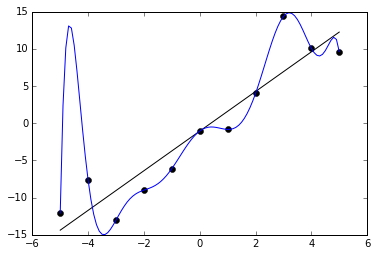
\includegraphics[width=0.7\textwidth]{Overfitted_Data.png}
\caption{A graph illustrating the concept of overfitting. The blue line goes through all of the known points (training data) very closely, but using this function to interpolate values between the known results is likely to produce very poor predictions. By contrast, the black line does not reproduce the training data precisely, but gives more accurate interpolation. Image Credit: \href{https://en.wikipedia.org/wiki/Overfitting}{Wikipedia}.}

\end{figure}

Overfitting can be caused by a poor choice of a number of parameters. Some of these are directly connected to the idea of overfitting. For example, in \verb|gap_config.cfg|, the first value in the variable \verb|default_sigma| is an estimate of the standard deviation in the energy calculations. This effectively tells the model how closely it should try to fit to the training data. A small value here will almost always lead to overfitting. However, sometimes other parameters can lead to overfitting in less obvious ways. For example, having extremely accurate descriptions of the atomic environments (determined by \verb|nmax| and \verb|lmax| in \verb|gap_config.cfg|) can lead to overfitting.

Note that if you want to save the GAP models you train with certain parameters, you will need to change the \verb|gp_file| keyword before you run \verb|gap_fit|, otherwise the model will be saved to \verb|gap.xml| every time, overwriting the previous model. However, if you do this you will also need to modify the python files you run to ensure that you load the correct model (all python files will load \verb|gap.xml| by default).

\subsubsection*{Exercises}

\begin{enumerate}
\item How could you identify when overfitting is taking place?
\item Using 100 training snapshots, train models using different values of \verb|default_sigma| for the energy and calculate the RMSE on the training and validation set each time. Do the results match your expectations? What is the optimal value, in your opinion?
\item (Optional) Repeat this exercise varying some of the other fitting parameters, \verb|cutoff|, \verb|atom_sigma|, \verb|nmax| and \verb|l_max|. Do these affect the accuracy of the model? Can they cause overfitting? What is the optimal value, in your opinion?
\item (Optional) Once you have found the optimal value of some parameter(s), use these parameters to train a model using 200 snapshots. Does this lead to more or less overfitting than when you used 100 snapshots? Is the difference significant?
\item What does this process teach you about what needs to be considered when efficiently training an ML model?

\end{enumerate}

%\subsection{Energy vs Forces}

%This section could be completed by just one member of your group.

\subsection{Running Molecular Dynamics with an ML Potential}
\label{sec:md}

%This section could be completed by just one member of your group.

So far we have only considered the energy predicted by the ML model, but the model also predicts the forces exerted on each atom by the electrons in the molecule. This means that once we have trained a machine learning model which we are happy is sufficiently accurate, we can use it to run molecular dynamics simulations. The simple script \verb|molecular_dynamics.py| does exactly that: it takes a snapshot from the validation set as a starting point, randomly assigns velocities to each atom, and uses the machine learned potential to calculate the forces acting on each atom. That is all of the information required to perform a dynamics simulation, as we use these velocities and forces to calculate the atomic positions and velocities a short time later, and then recalculate the forces on the atoms in their new positions using the ML potential. Doing this repeatedly results in a molecular dynamics trajectory.

\subsubsection*{Exercises}

\begin{enumerate}

\item Read through through the python script \verb|molecular_dynamics.py| and make sure you understand what each command does.
\item Run a molecular dynamics simulation for 200 timesteps at constant energy, and check the logfile \verb|nve.log| which is produced. What information in this log file could you use to establish if your ML potential is working as expected or not?
\item What is the microscopic reason that we see the temperature in the log file fluctuating over the course of the simulation?
\item Run a molecular dynamics simulation at constant temperature for 100 timesteps, and check the logfile \verb|nvt.log| which is produced. You will see that the total energy of the system is not conserved. What real-life experimental conditions are we reproducing which explains this variation in the total energy?
\item The dynamics calculated using the ML potential are approximately 1400 times faster than the traditional MD simulation I performed to obtain the training data. However, that doesn't account for the time it takes to create the model in the first place. What additional timings do we need to know to make a truly fair comparison of the computation costs of the two approaches? When will it be worth training an ML model to perform dynamics?

\end{enumerate}

\section{Learning Polarizabilities}

We can also use the data in the \verb|gap_input_N.xyz| files to train a ML model which can predict the polarizabilities of water snapshots. In these data files, the polarizability associated with each snapshot is listed along with the energies and forces; as with the ML potential, the atomic positions and their associated polarizabilities are all we need to train a suitable model.

Unlike the single command for training the ML model for the potential energy, the software to train the model which predicts polarizabilities needs to be run in stages. To make this process simpler, all the necessary commands have collected in a single file, \verb|polarizability.sh|, which is in the \verb|polarizability| folder. You can open this file using a text editor to modify the commands, and then run them all by typing \verb|./polarizability.sh| on the command line while in that folder.

%\subsection{Training a Model}

The first two commands in \verb|./polarizability.sh| calculate the descriptors describing each atomic environment present in the input file (\verb|-f $training_data|). It appears twice because we need the descriptors which transform as $L=0$ (\verb|-lm 0|) and those which transform as $L=0$ (\verb|-lm 2|). The systems are periodic (\verb|-p|), and we choose to keep the 200 most relevant features of each atomic environment (\verb|-nc 200|). The atomic environments are again defined by the cutoff radius (\verb|-rc 4.0|) and the width of the Gaussian centered on each atom (\verb|-sg 0.3|).

The next two commands simply take these descriptors and calculate the kernels which describe the similarity between each pair of atomic environments in the dataset, for both $L=0$ and $L=2$. There is no need to modify any of the parameters for these commands.

The final command both trains an ML model based on these descriptors and the polarizability data in the input file, and validates the model and outputs the results. In this case, no calculation of the error in the predicted polarizabilities of the training set is performed. The first three options indicate that the property to be learned is the Polarizability (\verb|-p Polarizabilility|), which is a rank 2 tensor (\verb|-r 2|) and symmetric (\verb|-t 1.0|). The next two options indicate the training data for the model, namely the atomic snapshots and their associated polarizabilities (\verb|-f $training_data|) and the kernels which relate the environments in these snapshots to one another (\verb|-k kernel0.npy kernel2.npy|). Then come the regularisation constants, which are introduced to prevent overfitting (\verb|-reg 1e-8 1e-5|, one for each kernel). Finally, the input file is split into a set of training and validation snapshots (\verb|-rdm 150|; 150 snapshots will be randomly selected to form the full training set, and the other 50 will be used for validation), and the number of training snapshots to use is selected (\verb|-ftr 0.1|; this means that 10\% of of selected 150 training snapshots will be used), and the polarizabilities of the validation set are predicted and compared to the true values (\verb|-pr|).

Note that this separation of commands means that you don't need to necessarily rerun every command for every new calculations. For example, if you wanted to test the performance of models trained with different numbers of training structures, then after you have calculated the descriptors and kernels for the first time, you will only need to rerun the command \verb|sagpr_train| with different parameters to achieve this. If you want to skip a command, simply place a \# at the start of its line in \verb|polarizability.sh| and it will not be executed.

\subsection*{Exercises}

\begin{enumerate}

\item Calculate a learning curve for three components of the polarizability ($xx$, $xy$, and $xx$). Would the model be further improved by adding more training structures?
\item Which components of the polarizability have similar learning curves? Why might this be the case?
\item We have kept only 200 features of each atomic environment in order to save space on our hard disk. Make a note of the size of the \verb|PS0.npy| and \verb|PS2.npy| files, then recalculate the learning curves from part 1 keeping 500 features of each atomic environment instead. Does this improve the accuracy of the ML models? How much bigger are the descriptor files in this case?
\item Try to optimize the ML model, varying the regularisation parameters and the definition of the atomic environments. What is the best strategy to perform this optimization? How accurate can you make your model?

\end{enumerate}

\subsection*{Predicting Polarizabilities of New Snapshots}

In Section \ref{sec:md} we calculated a short molecular dynamics trajectory using a ML potential we had trained. If we were using traditional quantum chemistry methods, we could have calculated the polarizabilities at the same time. When using ML, we need to use a separate ML model to predict the polarizabilities of each snapshot which we have generated, such as the one we have just trained. Therefore, we can now put everything together, and obtain a molecular dynamics trajectory with the associated polarizabilities using purely ML models.

The commands needed to do this are collected in the script \verb|prediction.sh| in the \verb|polarizability| folder. These are similar to the commands we have seen before: the first retrains the model using all 200 training structures (make sure you set the regularisation parameters here to whatever you found the optimal values to be before retraining). We then calculate the descriptors of the new snapshots and calculate the kernels which relate each new snapshot to the training snapshots. Finally we use the model we have trained (contained in the files \verb|weights_0.npy| and \verb|weights_2.npy|) to predict the polarizability of each new structures.

Run the prediction script: \verb|./prediction.sh|. The predicted polarizabilities should be saved in a new file \verb|trajectory_cartesian.out|. We don't have any reference values for these snapshots, since we only just generated them, but you can check that the values are at least similar to the polarizabilities in the training data by looking at the \verb|Polarizability| keyword in the comment lines of \verb|gap_input_200.xyz|.


\section{Summary}
You have now completed a full machine-learning driven molecular dynamics simulation! You trained a model to predict the energy and forces of water, optimising the various parameters which govern the models performance. You used that model to perform molecular dynamics simulations, at a fraction of the computational cost of a traditional simulation. And you trained a model to predict complex properties along that trajectory, in this case avoiding the need for post-DFT calculations. In principle, you can you use these methods (or very similar ones) to simulate the dynamics and properties of any type of material, provided you have enough high quality training data!


\end{document}
